\documentclass[10pt, usenames,dvipsnames, xcolor=table]{beamer}
\usepackage[utf8]{inputenc}
\usepackage{utopia}
\usepackage{lmodern}
\usepackage{graphicx}
\usepackage{amsmath}
\usepackage{nicefrac}
\usepackage{parskip}
\usepackage{media9}
\definecolor{UniBlue}{RGB}{0, 81, 149}
\setbeamercolor{structure}{fg=UniBlue}
\usetheme{Darmstadt}
\setbeamersize{text margin left=3mm,text margin right=3mm} 
\usepackage{gensymb}
\usepackage{mathtools}
\usepackage{hyperref}
\usepackage{graphicx}
\usepackage{longtable}
\usepackage{cancel}
\usepackage{multimedia}
\usepackage{resizegather}
\setcounter{MaxMatrixCols}{20}
\graphicspath{{Figures/}}

%------------------------------------------------------------
%This block of code defines the information to appear in the
%Title page

\makeatother
\setbeamertemplate{footline}
{
  \leavevmode%
  \hbox{%
  \begin{beamercolorbox}[wd=.2\paperwidth,ht=2.25ex,dp=1ex,center]{author in head/foot}%
    \usebeamerfont{author in head/foot}\insertshortauthor
  \end{beamercolorbox}%
  \begin{beamercolorbox}[wd=.8\paperwidth,ht=2.25ex,dp=1ex,center]{title in head/foot}%
    \usebeamerfont{title in head/foot}\insertshorttitle\hspace*{3em}
    \insertframenumber{} / \inserttotalframenumber\hspace*{1ex}
  \end{beamercolorbox}}%
  \vskip0pt%
}
\makeatletter
\setbeamertemplate{navigation symbols}{}

\usepackage{subfig}
\title{Steady-State Low-Order Explicit (LOE) Runge-Kutta Schemes with Improved Convergence}
\subtitle{AIAA Aviation}
\author[Z. Sabri, R. Hixon]{Zaid Sabri \\ Ray Hixon}
\institute[UT]
{
University of Toledo \\
Toledo Ohio, 43606 USA
}

\logo{%
    \includegraphics[width=1cm,height=0.5cm,keepaspectratio]{UT_shield.png}~%
    \includegraphics[width=1cm,height=0.5cm,keepaspectratio]{NASA.png}~%
}

\date{June 12 - 16, 2023}

\begin{document}

\frame{\titlepage}

\section{Introduction}
\begin{frame}{Background}
  \begin{columns}
    \column{1.0\textwidth}
      \begin{itemize}
        \item Computational Fluid Dynamics (CFD) is the study of fluid mechanics that predicts fluid
          flows using digital computers.
        \item To accomplish this goal, the analytic governing equations of fluid motion are
          discretized in space (using structured grid meshing), resulting in a system of coupled
          ordinary differential equations (ODE).
        \item ODE are integrated in the temporal direction using numerical integration schemes to
          advance the flow in time.
        \item The effectiveness of numerical integration depends on convergence, accuracy, and
          computational efficiency.
      \end{itemize}   
  \end{columns}
\end{frame}

\begin{frame}{Spatial Derivative}
  \begin{columns}
  \column{0.5\textwidth}
    \begin{itemize}
      \item Derivative of flow fluxes can be expressed with values of the function at the 
            neighboring point by using the Taylor series expansion. 
      \item The spatial derivative is calculated using a \textbf{finite difference} approach.
      \begin{equation*}
		    \begin{split}
			    \color{red}{\left.\frac{\partial{u}}{\partial{x}}\right|_{Numerical}}\color{black}{}~=&~
            \underbrace{\frac{\partial{u}}{\partial{x}}}_{\text{Exact}}\color{blue}
            {\underbrace{\left[\frac{\left(k^*\Delta{x}\right)}{\left(k\Delta{x}\right)}\right]}_{
            \text{Error}}}
		    \end{split}
		  \end{equation*}
    \end{itemize}
    \column{0.5\textwidth}
		\begin{figure}[htbp!]
		  \begin{center}
    	  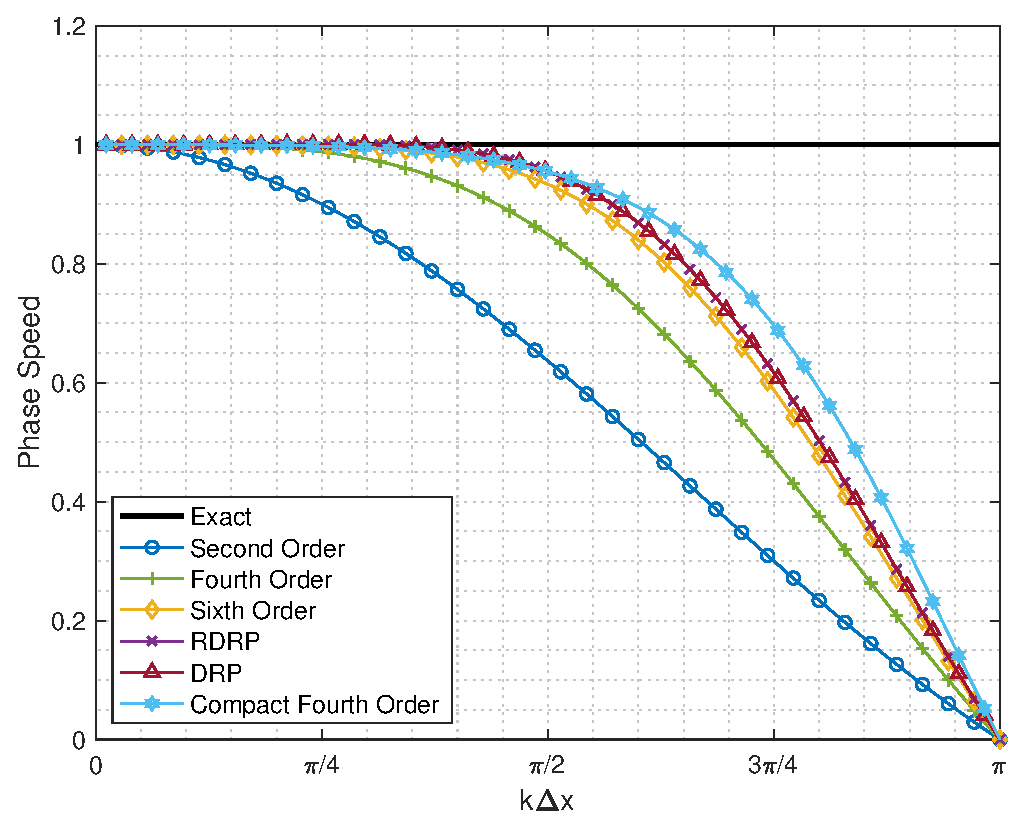
\includegraphics[width=1.0\textwidth]{Figures/Phase_Speed.eps}
    	\end{center}
		\end{figure} 
  \end{columns}
\end{frame}

\begin{frame}{Time Marching}
  \begin{columns}
    \column{1.0\textwidth}
    \begin{itemize}
      \item Starting with an initial state at time zero, given a boundary condition, we can 
            ”march” one time-step to a time later and use a numerical scheme to evaluate the 
            solution at that time.
      \item This process, known as time marching, can be used to obtain steady-state solutions 
            for steady flow problems and time-accurate solutions for unsteady flow problems.
      \item Time marching is subdivided into two schemes, \textbf{explicit} and \textbf{implicit}.
      \item Explicit schemes can be relatively simple to implement but may require excessive 
            time steps due to a bounded stability limit.
      \item When solving viscous flow problems where the computational domain must be highly 
            clustered near the body, the size of the time step an explicit scheme can take is 
            restricted by the CFL condition. 
      \item The stability restriction can be eliminated by using an implicit time marching scheme.
    \end{itemize}   
  \end{columns}
\end{frame}

\section{Implicit Time Marching}
\begin{frame}{Implicit Time Marching}
  \begin{columns}
    \column{1.0\textwidth}
    \begin{itemize}
      \item To derive the implicit time marching algorithm, the one-dimensional Euler equation 
            can be written as:
 			\begin{equation}
				\begin{split}
					\label{eq:Implicit_Scheme}
  					\frac{\partial{Q}}{\partial{t}}
            +\left.\frac{\partial{E}}{\partial{x}}\right|^{n+1}~=~0
				\end{split}
			\end{equation}
      \item Linearize the Taylor Series expansion of the fluxes to rewrite the delta form of the
            equation as:
      \begin{equation}
        \underbrace{\left[I+\frac{\partial}{\partial{x}}\left(\Delta{t}\cdot
        \left.\frac{\partial{E}}{\partial{Q}}\right|_{i}^n
        \right)\right]}_{\text{{\color{red}{Numerics}}}}\left\{\Delta{Q_{i}}\right\}~=~
        -\Delta{t}\cdot
        \underbrace{\left\{\frac{\partial}{\partial{x}}\left(E_{i}^n
        \right)\right\}}_{\text{Physics}}            
      \end{equation}
    \item Much research has focused on approximating the {\color{red}{Numerics}} due to complexities 
        involved with inverting an unfactored implicit scheme in multi-dimensions.
    \end{itemize}   
  \end{columns}
\end{frame}

\begin{frame}\frametitle{Implicit Time Marching - Prior Work}
  \begin{columns}
  \column{1.0\textwidth}
    \begin{itemize}
      \item \textbf{Alternating Direction Implicit} (ADI) is a practical implicit scheme that 
            approximately factorizes the implicit operator in delta form.
      \item The \textbf{Lower-Upper Symmetric-Gauss-Seidel} method (LU-SGS) is another common 
          approximation where the numerics are preconditioned to a product of three matrices which 
          provides computational efficiency.
      \item A preconditioner, pseudo-time derivative, can be added to the equations to accelerate
        the time evolution scheme in the unsteady equation, an algorithm first proposed by Anthony
        Jameson is known as \textbf{Dual-Time Stepping}.
      \item Implicit time marching has been introduced with higher-order differencing stencils
            by Miguel Visbal and Datta Gaitonde from the Air Force Research Lab and Ohio State 
            University, \textbf{FDL3DI}.
    \end{itemize}  
  \end{columns}
\end{frame}

\begin{frame}{Implicit Time Marching - Preconditioning}
  \begin{columns}
  \column{1.0\textwidth}
    \begin{itemize}
		  \item Instead of using:
      \begin{equation}
	      \label{eq:RDRP_NS}\resizebox{0.85\hsize}{!}{$%
  		  \left[I+\Delta{t}\left(\frac{A_{i+3}-8A_{i+2}+37A_{i+1}-37A_{i-1}+8A_{i-2}-A_{i-3}}
        {48\Delta{x}}\right)^{n+1,l}\right]\Delta{Q}_i~=~-\Delta{t}\left\{RHS\right\}_i^{n+1,l}$}
      \end{equation}
      Is preconditioned as follows:
      \begin{equation}
      	\label{eq:TriDi_NS}
        		\left[I+\Delta{t}\left(\frac{A_{i+1}-A_{i-1}}{2\Delta{x}}\right)^{n+1,l}\right]
            \Delta{Q}_i~=~-\Delta{t}\left\{RHS\right\}_i^{n+1, l}
      \end{equation}
		  \item This will result in a more efficient solver since the number of diagonals has been 
            reduced.
    \end{itemize}  
  \end{columns}
\end{frame}

\begin{frame}{Stability}
  \begin{columns}
    \column{1.0\textwidth}
    \begin{itemize}
      \item The equation is changed to add a scaling factor $\color{red}{\sigma}$ multiplying the 
            spatial derivative on the LHS:
      \begin{equation}
        		\left[I+\Delta{t}{\color{red}{\sigma}}
            \left(\frac{A_{i+1}-A_{i-1}}{2\Delta{x}}\right)^{n+1,l}\right]\Delta{Q}_i~=~
            -\Delta{t}\left\{RHS\right\}_i^{n+1, l}
      \end{equation}
      \begin{table}[htp!]
        \centering
        \resizebox{0.9\textwidth}{!}{%
        \begin{tabular}{|l|c|c|c|c|c|c|}
        \hline & 
          \multicolumn{1}{c|}{\textbf{$\sigma_{E2}$}} & 
          \multicolumn{1}{c|}{\textbf{$\sigma_{E4}$}} & 
          \multicolumn{1}{c|}{$\sigma_{E6}$} & \multicolumn{1}{c|}{$\sigma_{DRP}$} & 
          \multicolumn{1}{c|}{$\sigma_{RDRP}$}& \multicolumn{1}{c|}{$\sigma_{C4}$}\\ \hline
        \textbf{Periodic} & \textit{1.0} & \textit{1.0} & \textit{$\nicefrac{11}{10}$} & 
        \textit{1.16682} & \textit{$\nicefrac{7}{6}$} & \textit{1.49982}\\ \hline
        \textbf{Bounded} & \textit{1.0} & \textit{2.121796} & \textit{6.352796} & 
        	\textit{4.9748714} & 
        	\textit{6.3620687} & 
        	\textit{3.80018}\\ \hline
        \end{tabular}%
        }
        \label{tab:Scaling}
      \end{table}
    \end{itemize}   
  \end{columns}
\end{frame}


\section{Results and Analysis}
\begin{frame}{Numerical Results for Benchmark Problems}
  \begin{columns}
    \column{0.5\textwidth}
      \begin{itemize}
        \item One Problem from the Third Computational Aeroacoustics (CAA) workshop is analyzed
              to validate the work done.
        \begin{equation*}
          \left(\begin{matrix}
              \frac{\partial{}}{\partial{t}} 
              \left\{\begin{matrix}
                  \rho \\
                  \rho{u} \\
                  E_{tot}
            \end{matrix}\right\}\\
             +\frac{\partial{}}{\partial{x}}
              \left\{\begin{matrix}
                  \rho{u} \\
                  \rho{u^2}+p \\
                  u(E_{tot}+p)
            \end{matrix}\right\} \\
            +\color{RedOrange}{\frac{1}{A}\frac{\partial{A}}{\partial{x}}}\color{black}{}
              \left\{\begin{matrix}
                  \rho{u} \\
                  \rho{u^2} \\
                  u(E_{tot}+p)
            \end{matrix}\right\}
          \end{matrix}\right)= 0
        \end{equation*} 
      \end{itemize}   
    \column{0.5\textwidth}
      \begin{figure}[hbt!]
          \centering
          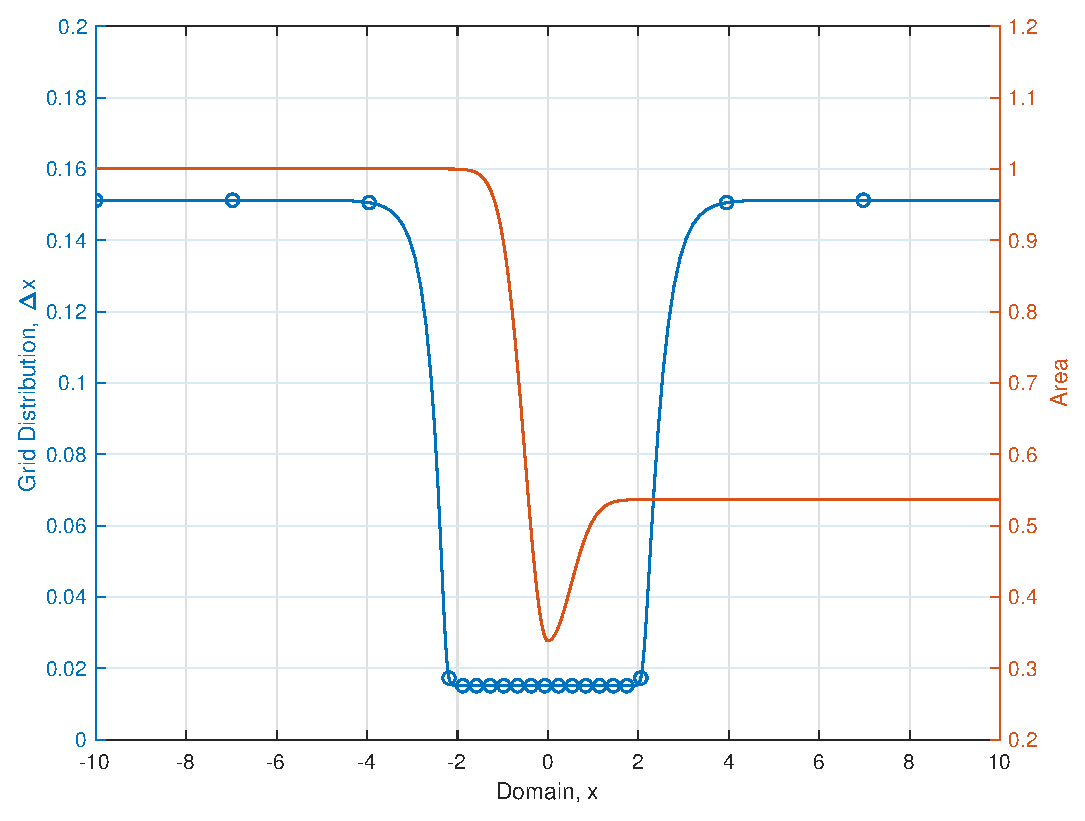
\includegraphics[width=1.0\textwidth]{Figures/Area_dX}
          \label{fig:Euler_CD_Area}
      \end{figure}
  \end{columns}
\end{frame}

\begin{frame}{Category 1 Problem 1, Steady State Results}
  \begin{columns}
    \column{1.0\textwidth}
    \begin{itemize}
      \item The mean flow is set as:
      \begin{equation*}
        \left\{
      	\begin{matrix}
      		\overline{\rho} \\
      		\overline{u} \\
      		\overline{p}
      	\end{matrix}
      	\right\}~=~
      	\left\{
      	\begin{matrix}
      		1.0 \\
      		0.4 \\
      		\frac{1}{\gamma}
      	\end{matrix}
      	\right\}
      \end{equation*}
    \end{itemize}
    \begin{figure}
      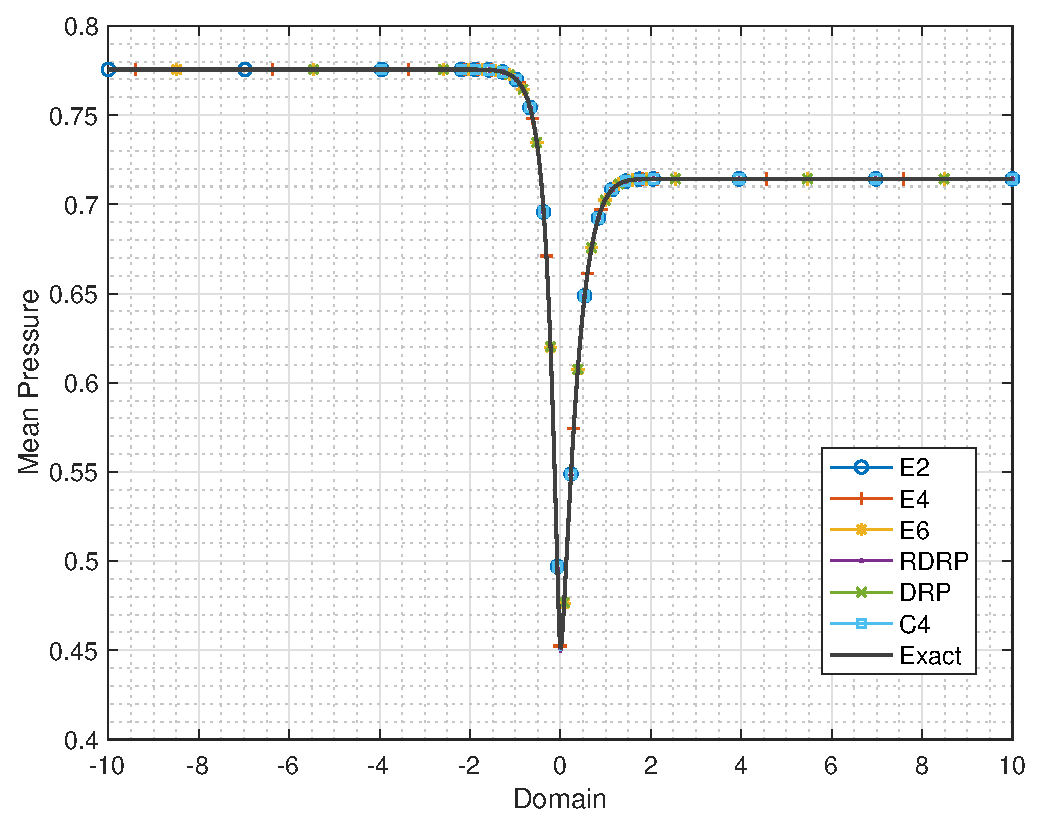
\includegraphics[width=0.48\linewidth]{Figures/C1P1_SteadyState}%
      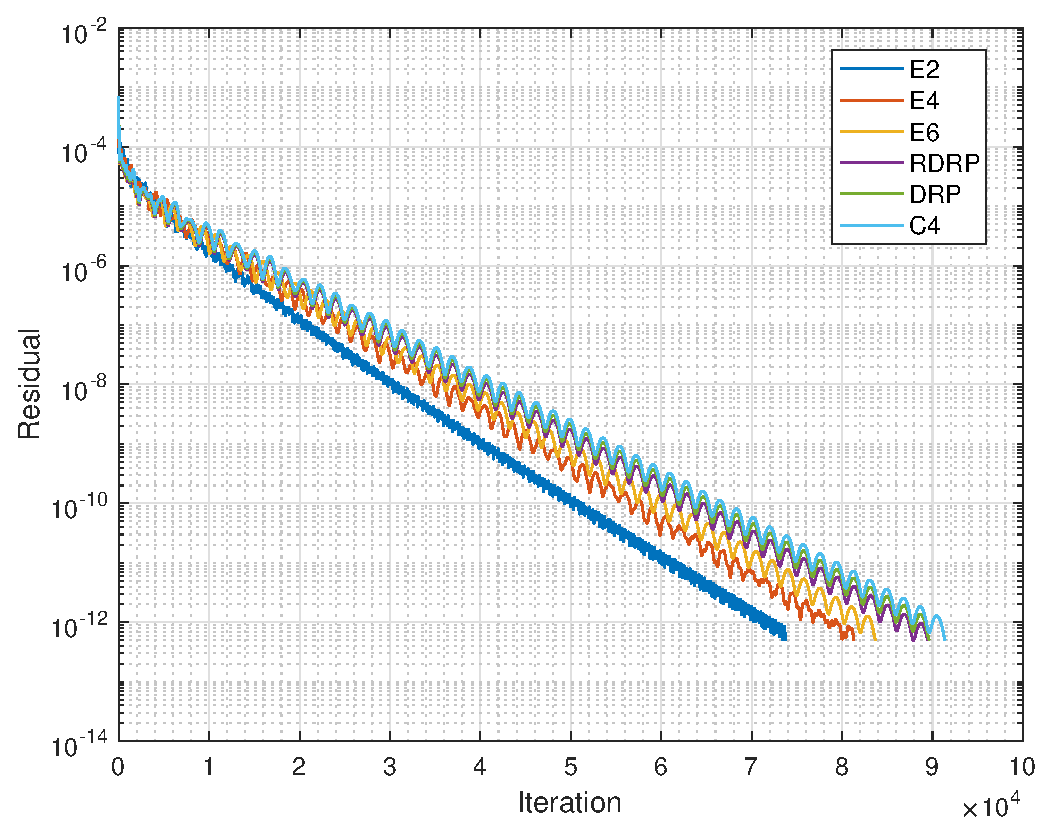
\includegraphics[width=0.48\linewidth]{Figures/C1P1_TriDi_Scaling_ROC}
    \end{figure}
  \end{columns}
\end{frame}

\begin{frame}{Category 1 Problem 1, Unsteady Results}
  \begin{columns}
    \column{1.0\textwidth}
    \begin{table}[htp!]
    \centering
    \label{tab:C1P1_CFL}
      \begin{tabular}{|l|c|c|c|c|c|c|}
      \hline & \multicolumn{1}{c|}{\textbf{E2}} & 
      \multicolumn{1}{c|}{\textbf{E4}} & 
      \multicolumn{1}{c|}{\textbf{E6}} & 
      \multicolumn{1}{c|}{\textbf{DRP}} & 
      \multicolumn{1}{c|}{\textbf{RDRP}}& 
      \multicolumn{1}{c|}{\textbf{C4}}\\ \hline
      \textbf{$\nu_{physical}$} & 
      \textit{12.521} & 
      \textit{17.518} & 
      \textit{19.858} & 
      \textit{20.834} & 
      \textit{20.834} & 
      \textit{22.237}\\ \hline
      \end{tabular}
    \end{table}
    ~~ \newline
    \begin{figure}[hbtp!]
    	\centering
    	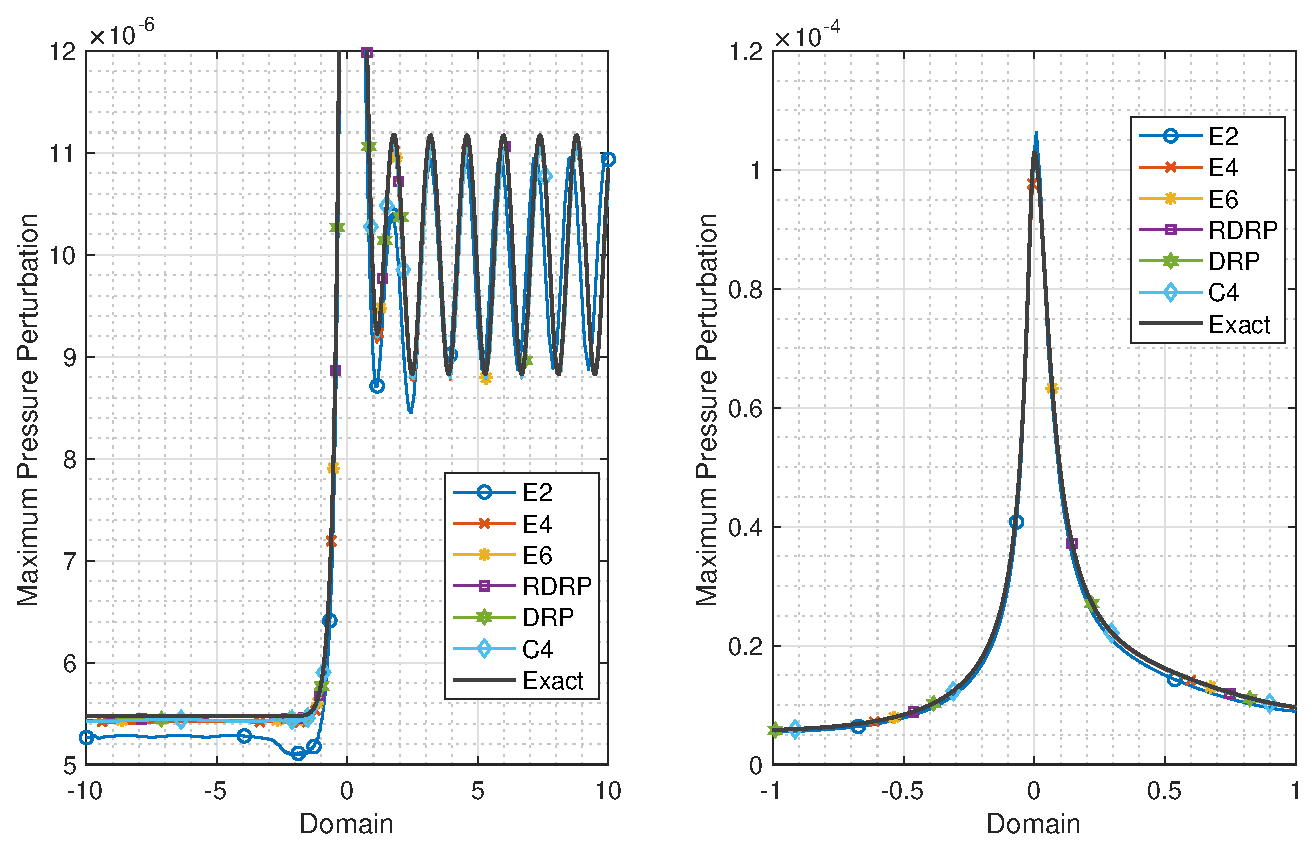
\includegraphics[width=1.0\textheight]{Figures/C1P1_MaxDisturbance_zoom}
    	\label{fig:Unsteady_C1P1}
    \end{figure}
  \end{columns}
\end{frame}


\section{Conclusions and Future Work}
\begin{frame}{Conclusion}
  \begin{columns}
    \column{1.0\textwidth}
    \begin{itemize}
      \item The present research aimed to establish a highly efficient implicit solver while
        using higher-order spatial differencing schemes. 
      \item Through scaling factors, the LHS matrix was replaced with an easier-to-solve matrix,
        cutting down on the computational work needed for the iterative steady-state solver. 
      \item Although the current study is based on one-dimensional problems, the findings
        suggest stability is possible if scaling factors are used on the LHS spatial difference.
      \item The preconditioned matrix was tested against steady and unsteady CAA workshop data;
        the numerical solution agrees well with the exact.  
    \end{itemize}
  \end{columns}
\end{frame}

\begin{frame}{Acknowledgments}
  \begin{columns}
  \column{1.0\textwidth}
        \begin{itemize}
        \item This work is supported by the NASA Advanced Air Transportation Technologies (AATT)
          Project. 
        \item The authors would like to thank Dr. Edmane Envia of the NASA Glenn Research Center,
          who is the technical monitor of this work.
        \end{itemize}
        \begin{block}{}
        	Zaid Sabri \\
        	The University of Toledo \\
        	Toledo Ohio, 43606 USA \\
        	+1 (567)377-9009 \\
        	zaid.sabri@rockets.utoledo.edu
        \end{block}
  \end{columns}
\end{frame} 
    
\end{document}
